% !TEX program = lualatex
\documentclass[a4paper,11pt]{ltjsarticle}

\usepackage[haranoaji]{luatexja-preset}
\usepackage{fontspec}
\setmainfont{TeX Gyre Pagella}
\setsansfont{TeX Gyre Heros}
\setmonofont{Latin Modern Mono}[Scale=0.86,BoldFont={Latin Modern Mono}]

\usepackage[a4paper,top=25mm,bottom=24mm,left=22mm,right=22mm,headheight=28pt]{geometry}
\usepackage{amsmath,amssymb,mathtools}
\usepackage{booktabs,tabularx,longtable,array,colortbl}
\usepackage{enumitem}
\usepackage{xcolor}
\usepackage{graphicx}
\usepackage{tikz}
\usetikzlibrary{arrows.meta,positioning,fit,shapes.geometric,calc,backgrounds}
\usepackage[most]{tcolorbox}
\usepackage{listings}
\usepackage{xurl}
\usepackage{hyperref}
\usepackage{bookmark}
\usepackage{fancyhdr}
\usepackage{titlesec}
\usepackage{caption}
\usepackage{placeins}
\usepackage{lastpage}

\definecolor{TFNavy}{HTML}{102A43}
\definecolor{TFBlue}{HTML}{1261A0}
\definecolor{TFCyan}{HTML}{2CB1BC}
\definecolor{TFMint}{HTML}{D9F2F0}
\definecolor{TFGold}{HTML}{D69E2E}
\definecolor{TFRed}{HTML}{C53030}
\definecolor{TFGreen}{HTML}{2F855A}
\definecolor{TFInk}{HTML}{243B53}
\definecolor{TFMuted}{HTML}{627D98}
\definecolor{TFPaper}{HTML}{F8FAFC}
\definecolor{TFLine}{HTML}{CBD5E0}
\definecolor{TFPurple}{HTML}{6B46C1}

\hypersetup{
  colorlinks=true,
  linkcolor=TFBlue,
  citecolor=TFBlue,
  urlcolor=TFBlue,
  pdftitle={TheoremForces L1 White Paper},
  pdfauthor={TheoremForces Project},
  pdfsubject={Kernel acceptance and independently verifiable Lean certificates},
  pdfkeywords={Lean, kernel, formal proof, axiom policy, certificate, reproducibility}
}

\pagestyle{fancy}
\fancyhf{}
\fancyhead[L]{\sffamily\small\color{TFMuted}TheoremForces L1 White Paper}
\fancyhead[R]{\sffamily\small\color{TFMuted}Version 0.3.0 - 2026-08-09}
\fancyfoot[L]{\sffamily\footnotesize\color{TFMuted}Audited L1 specification - issuance disabled}
\fancyfoot[R]{\sffamily\footnotesize\color{TFMuted}\thepage\ / \pageref{LastPage}}
\renewcommand{\headrulewidth}{0.4pt}
\renewcommand{\headrule}{\hbox to\headwidth{\color{TFLine}\leaders\hrule height \headrulewidth\hfill}}

\titleformat{\section}
  {\sffamily\Large\bfseries\color{TFNavy}}
  {\thesection}{0.75em}{}
\titleformat{\subsection}
  {\sffamily\large\bfseries\color{TFBlue}}
  {\thesubsection}{0.65em}{}
\titleformat{\subsubsection}
  {\sffamily\normalsize\bfseries\color{TFInk}}
  {\thesubsubsection}{0.55em}{}
\titlespacing*{\section}{0pt}{2.2ex plus 0.6ex}{1.0ex}
\titlespacing*{\subsection}{0pt}{1.8ex plus 0.4ex}{0.7ex}

\setlist[itemize]{leftmargin=1.6em,itemsep=0.35em,topsep=0.4em}
\setlist[enumerate]{leftmargin=1.8em,itemsep=0.35em,topsep=0.4em}
\setlength{\parindent}{1em}
\setlength{\parskip}{0.32em}
\renewcommand{\arraystretch}{1.24}
\captionsetup{font=small,labelfont={bf,color=TFNavy}}
\setcounter{tocdepth}{2}

\newcolumntype{Y}{>{\raggedright\arraybackslash}X}
\newcolumntype{L}[1]{>{\raggedright\arraybackslash}p{#1}}
\newcommand{\term}[1]{\textbf{\color{TFNavy}#1}}
\newcommand{\code}[1]{\texttt{#1}}
\newcommand{\pass}{\textcolor{TFGreen}{\textbf{PASS}}}
\newcommand{\fail}{\textcolor{TFRed}{\textbf{FAIL}}}
\newcommand{\unknown}{\textcolor{TFGold}{\textbf{UNKNOWN}}}
\newcommand{\glossref}[2]{\hyperlink{glossary:#1}{#2}}

\newtcolorbox{principlebox}[1]{
  enhanced,breakable,colback=TFMint!42,colframe=TFCyan,
  boxrule=0.7pt,arc=2mm,left=3mm,right=3mm,top=2mm,bottom=2mm,
  title={#1},fonttitle=\sffamily\bfseries,coltitle=TFNavy
}
\newtcolorbox{warningbox}[1]{
  enhanced,breakable,colback=TFRed!4,colframe=TFRed!75,
  boxrule=0.7pt,arc=2mm,left=3mm,right=3mm,top=2mm,bottom=2mm,
  title={#1},fonttitle=\sffamily\bfseries,coltitle=TFRed
}
\newtcolorbox{atomicgatebox}[1]{
  enhanced,colback=TFRed!4,colframe=TFRed!75,
  boxrule=0.7pt,arc=2mm,left=3mm,right=3mm,top=2mm,bottom=2mm,
  title={#1},fonttitle=\sffamily\bfseries,coltitle=TFRed
}
\newtcolorbox{decisionbox}[1]{
  enhanced,breakable,colback=TFBlue!4,colframe=TFBlue!80,
  boxrule=0.7pt,arc=2mm,left=3mm,right=3mm,top=2mm,bottom=2mm,
  title={#1},fonttitle=\sffamily\bfseries,coltitle=TFNavy
}
\newtcolorbox{specbox}[1]{
  enhanced,breakable,colback=TFPaper,colframe=TFPurple!80,
  boxrule=0.8pt,arc=2mm,left=3mm,right=3mm,top=2mm,bottom=2mm,
  title={#1},fonttitle=\sffamily\bfseries,coltitle=TFPurple
}

\lstdefinelanguage{Lean}{
  morekeywords={theorem,lemma,def,example,namespace,end,import,by,fun,forall,where,let,in,if,then,else,match,with,open,variable,structure,class,inductive,abbrev,exact,intro,rw,simp,have,show,set_option,axiom},
  sensitive=true,morecomment=[l]{--},morestring=[b]"
}
\lstdefinelanguage{JSON}{
  morestring=[b]",showstringspaces=false,
  literate={:}{{{\color{TFInk}:}}}{1} {,}{{{\color{TFInk},}}}{1}
}
\lstset{
  language=Lean,basicstyle=\ttfamily\footnotesize,
  keywordstyle=\color{TFBlue}\bfseries,commentstyle=\color{TFMuted}\itshape,
  stringstyle=\color{TFGreen},backgroundcolor=\color{TFPaper},
  frame=single,rulecolor=\color{TFLine},framesep=5pt,
  xleftmargin=4pt,xrightmargin=4pt,breaklines=true,
  showstringspaces=false,columns=fullflexible,keepspaces=true
}

\begin{document}

\hypersetup{pageanchor=false}
\begin{titlepage}
\thispagestyle{empty}
\begin{tikzpicture}[remember picture,overlay]
  \fill[TFNavy] (current page.north west) rectangle ([yshift=-115mm]current page.north east);
  \fill[TFCyan] ([yshift=-115mm]current page.north west) rectangle ([yshift=-118mm]current page.north east);
  \node[draw=TFCyan,line width=1.3pt,rounded corners=3mm,minimum width=31mm,minimum height=31mm,
        text=white,font=\sffamily\bfseries\fontsize{22}{22}\selectfont]
        at ([xshift=-34mm,yshift=-35mm]current page.north east) {L1};
  \foreach \x/\y in {28/29,52/43,79/27,107/48,137/31,163/51}{
    \fill[TFCyan!70] ([xshift=\x mm,yshift=-\y mm]current page.north west) circle (1.5mm);
  }
  \draw[TFCyan!55,line width=0.8pt]
    ([xshift=28mm,yshift=-29mm]current page.north west) --
    ([xshift=52mm,yshift=-43mm]current page.north west) --
    ([xshift=79mm,yshift=-27mm]current page.north west) --
    ([xshift=107mm,yshift=-48mm]current page.north west) --
    ([xshift=137mm,yshift=-31mm]current page.north west) --
    ([xshift=163mm,yshift=-51mm]current page.north west);
\end{tikzpicture}

\vspace*{17mm}
{\sffamily\bfseries\fontsize{15}{18}\selectfont\color{TFCyan} THEOREMFORCES}\par
\vspace{8mm}
{\sffamily\bfseries\fontsize{30}{37}\selectfont\color{white}
L1: Kernel Acceptance\par
仕様と検証アーキテクチャ}\par
\vspace{5mm}
{\sffamily\fontsize{14}{19}\selectfont\color{white!83}
An Independently Verifiable Foundation for Lean Certificates}\par

\vspace{32mm}
\begin{tcolorbox}[
  colback=white,colframe=TFLine,boxrule=0.6pt,arc=2mm,
  left=5mm,right=5mm,top=4mm,bottom=4mm]
\textbf{Status}\quad Audited design specification\hfill
\textbf{Version}\quad 0.3.0\hfill
\textbf{Date}\quad 2026-08-09

\medskip
本書は TheoremForces の assurance model のうち、最下層かつ不可欠な
\term{L1: kernel acceptance} だけを独立して定義する。Lean kernel による型検査、
exact artifact と対象定理の拘束、axiom policy、fail-closed な判定、証明書 schema、
独立検証、脅威モデル、および実装 gate を規定する。

\medskip
\textbf{0.3.0 security revision:} hostile Lean process を acceptance authority から外し、trusted Challenge +
Comparator、sandbox 外 proof export、Lean checker + independent checker quorum、cycle-free signed envelope、
exact artifact manifest、production Gate 0--C を normative に固定した。Gate C 完了まで L1 issuance は無効である。
\end{tcolorbox}

\vfill
{\sffamily\large\bfseries\color{TFNavy}TheoremForces Project}\par
{\sffamily\color{TFMuted}\url{https://theoremforces.org/}}\par
\vspace{5mm}
{\footnotesize\color{TFMuted}
Independent project. Not affiliated with, endorsed by, or sponsored by Lean FRO,
the Lean project, or the mathlib maintainers.}
\end{titlepage}

\hypersetup{pageanchor=true}
\pagenumbering{roman}

\begin{tcolorbox}[
  colback=TFNavy,colframe=TFNavy,arc=2mm,
  left=5mm,right=5mm,top=4mm,bottom=4mm]
{\sffamily\bfseries\large\color{white}要旨}

\color{white!92}
L1 は「提出された文字列がもっともらしい」ことではなく、固定された環境において、
指定された Lean declaration が trusted Challenge と一致し、exported proof term を official Lean checker と
independent checker の quorum が受理したことを表す。
ただし kernel は、import 済みの定数や公理を前提として導出可能性を判定するため、
受理そのものと axiom policy への適合は区別しなければならない。

TheoremForces の operational L1 は、checker quorum に加えて、exact source hash、
environment digest、target declaration、依存閉包、axiom report、実行状態を同一 certificate に拘束する。
受理経路が一つでも不明なら L1 を発行しない。第三者は署名や UI を信用せず、artifact と環境を取得し、
同じ判定を再実行できる。本書はこの最小構成を検証可能な仕様として提示する。
\end{tcolorbox}

\section*{Abstract}
L1 denotes a narrow claim: in an identified Lean environment, the exported proof term associated with a
trusted-challenge-bound declaration was accepted by both the pinned Lean checker and an independent checker.
This is a claim of derivability relative to
the imported environment, not a claim that the formal statement matches an informal intention, is
novel, useful, axiom-free, or authored by a particular person.

TheoremForces operationalizes L1 by binding trusted challenge comparison and checker-quorum acceptance to an exact source artifact, exactly
one target declaration, environment digest, primitive axiom set, certificate dependency closure, resource outcome, and an
append-only certificate record. The design is fail-closed: an ambiguous target, incomplete axiom
report, artifact mismatch, timeout, or infrastructure error cannot be represented as acceptance.
An independent verifier can reconstruct and replay the judgment without trusting the website.

\begin{decisionbox}{Normative language and scope}
The words \term{MUST}, \term{MUST NOT}, \term{SHOULD}, and \term{MAY} express requirements in this
design specification. Version 0.3 normative correction、Sections 3--10、requirement catalog、Gate 0--C、
versioned schema / golden vectors / adversarial fixtures are normative unless explicitly marked informative. The
document is version-neutral with respect to Lean and Mathlib: every concrete certificate identifies
its own environment rather than relying on a moving notion of ``current.''
\end{decisionbox}

\tableofcontents
\clearpage
\pagenumbering{arabic}

\section{Version 0.3 normative security correction}

\begin{warningbox}{NO-GO until Gate C}
通常の \code{lean} process と human-readable axiom output は hostile proof marketplace の acceptance authority に
できない。Version 0.2 で未決定だった type serialization、canonical JSON、signature、artifact root、checker boundary、
registry retention は本節で固定する。本節と後続節が衝突する場合は本節を優先する。Gate 0--C 完了前は site を
deploy してもよいが、新規 \term{L1 accepted} issuance は MUST remain disabled であり、historical v1 record は
\code{legacy-incomplete} と表示する。
\end{warningbox}

\subsection{Current production persistence boundary}

2026-08-09 時点の production web は Cloudflare D1 を Prisma D1 adapter 経由で使用する。この adapter 経路は、
certificate issuance、accepted transition、economy / reputation credit、ledger event、bounty settlement にまたがる
multi-row mutation に必要な atomic multi-statement transaction を提供しない。したがって current deployment の
trust-critical public acceptance / issuance surface は write-disabled であり、公開側には public browsing と historical
record の表示だけを提供する。新規 L1 issuance、関連 credit / ledger / bounty mutation、judge queue delivery は fail-closed
に保つ。これは application の全 write を禁止する主張ではない。Private draft 保存、registry の non-issuance maintenance、
API の non-issuance write は分離した boundary で継続し得るが、L1 acceptance または issuance-coupled side effect を生成・変更
してはならない。この停止は Gate C 合格を意味せず、L1-ATOM-001 の release evidence が揃うまで解除しない。

\subsection{Hostile Lean and checker quorum}

User-controlled Lean source、macro、command、tactic、plugin、import、\code{.olean} は hostile input である。
\code{debug.skipKernelTC}、unchecked environment mutation、malicious meta-program を含む通常 build の exit 0 は builder
evidence にすぎず、L1 を単独で成立させない。Issuer から分離した verifier domain は次をすべて MUST verify する。

\begin{enumerate}
  \item Organizer-controlled trusted Challenge artifact digest と submitted declaration の equality を pinned Comparator で確認する。
  \item Builder sandbox から proof export を取り出し、sandbox 外の no-user-code verifier へ渡す。
  \item Pinned official Lean checker と、異なる implementation / code base の independent checker の両方で export を検査する。
  \item Type、value、universe parameters、declaration kind、proof export、transitive axiom closure の digests を再計算する。
  \item 一方でも reject、crash、timeout、unsupported、diverge なら accepted にせず、rejected または indeterminate とする。
\end{enumerate}

Initial independent checker profile は policy で pin した nanoda-compatible checker とする。対象 feature が未対応なら
quorum を弱めず issuance を止める。Comparator、Lean checker、exporter、independent checker の source commit、binary
digest、build provenance を logical environment manifest に含める。Lean の untrusted-proof validation guidance と
Comparator model を trust boundary の根拠とする\cite{leanvalidate,leancomparator}。

\subsection{Normative requirement catalog}

各 requirement は repository の machine-readable catalog に同じ ID、owner、conformance test、release evidence URI を
持つ。Unknown、skipped、flaky、manual-only は PASS ではない。

\begin{longtable}{@{}L{28mm}L{127mm}@{}}
\toprule
\textbf{ID} & \textbf{Normative requirement} \\
\midrule
\endfirsthead
\toprule
\textbf{ID} & \textbf{Normative requirement (continued)} \\
\midrule
\endhead
L1-CONF-001 & 全 MUST に stable ID、automated test、versioned fixture、release evidence が存在する。 \\
L1-ACC-001 & Accepted は本 catalog の必須 subpredicate の conjunction のみであり、missing / unknown は fail-closed。 \\
L1-TRUST-001 & Hostile build は non-root、no-secret、read-only input、fresh workspace、default-deny egress、zero capability、seccomp、PID / mount / user namespace または microVM 内だけで実行する。 \\
L1-VER-001 & \code{debug.skipKernelTC}、unchecked \code{addDecl}、malicious meta-code fixture は accepted にならない。 \\
L1-VER-002 & Trusted Challenge digest と Comparator equality が必須。Statement substitution は reject する。 \\
L1-VER-003 & Lean checker と independent checker quorum が PASS。一方の reject / crash / unsupported は非 accepted。 \\
L1-VER-004 & Sandbox 外で validated proof export を検査し、その digest を CertificateCore に拘束する。 \\
L1-TGT-001 & Challenge artifact / statement は organizer-controlled CAS object として dispatch 前に固定する。 \\
L1-TGT-002 & Environment delta 上の user target は exactly one。Macro-generated second declaration、\code{opaque}、\code{axiom}、\code{run\_cmd} injection を reject する。 \\
L1-TGT-003 & Fully qualified name、kind、universe parameters、type / value / proof-export digest を記録し replay で一致させる。 \\
L1-ART-001 & Raw upload、decoded entrypoint、canonical manifest、bundle root、generated source を別 digest / insert-only CAS object として保存する。 \\
L1-ART-002 & Canonical path profile を固定し、absolute / dot / dot-dot / backslash / NUL / case-fold collision / symlink / hardlink / special file を reject する。 \\
L1-ART-003 & Build 中 input は immutable で pre / post bundle root が一致する。 \\
L1-ENV-001 & Toolchain、imports、binary、image platform、command、option、SBOM、provenance の全 identity を manifest 化する。 \\
L1-ENV-002 & Moving tag、network resolution、unmanifested file access、shared mutable cache を禁止する。 \\
L1-ENV-003 & Known-unsound / advisory-blocked epoch では exact pin にかかわらず issuance を停止する。 \\
L1-AX-001 & Proof export から structured transitive axiom closure を verifier domain で独立再計算する。 \\
L1-AX-002 & Primitive baseline は exact declaration identity、kind、type digest、origin module digest で固定する。 \\
L1-AX-003 & \code{sorryAx}、compiler trust、native computation由来、custom / unknown assumption を deny する。 \\
L1-REG-001 & Certified dependency は real proof export または全 upstream checker receipt、type / value / export digest に拘束する。 \\
L1-REG-002 & DAG、issuance-before dependency checkpoint、status-at-checkpoint、current status、taint closure を検証する。 \\
L1-CERT-001 & Strict JSON Schema、RFC 8785 JCS、I-JSON constraints、cross-language golden vectors を使う。 \\
L1-CERT-002 & CertificateCore、IssuanceAttestation、LogReceipt を分離し、Ed25519 domain-separated non-self-referential envelope を使う。 \\
L1-CERT-003 & Required field 欠落、unknown field、duplicate key、bad Unicode、bad digest / timestamp / size を reject する。 \\
L1-LOG-001 & Cumulative log inclusion / consistency proof、signed checkpoint、two independent witness receipts を metadata verifier が検証する。 \\
L1-KEY-001 & Key validity、algorithm、role、rotation、revocation を issuance checkpoint に対して検証する。 \\
L1-RUN-001 & Limit と actual CPU / wall / RSS / PID / file / disk / inode / output / network、exit / signal / OOM / timeout / truncation を記録する。 \\
L1-RUN-002 & Exit 0、expected structured result exactly once、no truncation、全 checker PASS が accepted の必須条件。 \\
L1-FAIL-001 & \code{accepted|rejected|indeterminate} と versioned reason precedence を固定し、attempt receipt と certificate を分ける。 \\
L1-FAIL-002 & Terminal transition は conditional DB write で atomic かつ一度。Duplicate / late callback は state を変えない。 \\
L1-ATOM-001 & Certificate、terminal state、economy / reputation credit、ledger event、bounty settlement の multi-row mutation は一つの atomic persistence boundary で commit する。Prisma D1 adapter の個別 write 列を transaction と扱わず、選定した atomic design が crash / retry / concurrent-finalize test に合格するまで issuance と全付随 mutation を fail-closed にする。 \\
L1-REP-001 & Verifier default は non-executing metadata mode。\code{--replay} は explicit opt-in と強制 sandbox を要求する。 \\
L1-RET-001 & Accepted certificate の全 replay object、failure attempt、event、receipt を lifetime 中取得可能にする。欠落時は \code{replay-unavailable} event を追記する。 \\
L1-UNI-001 & Source bytes は非正規化で hash し、UI は bidi / control / default-ignorable を可視化して escaped byte view を提供する。 \\
L1-OPS-001 & False acceptance、checker divergence、artifact mismatch、log fork、key incident で 5 分以内に automatic issuance pause。 \\
L1-OPS-002 & Gate C の 30 日観測完了まで production L1 issuance を禁止する。 \\
L1-TEST-001 & Adversarial corpus、clean-host replay、second-operator replay を release gate にする。 \\
\bottomrule
\end{longtable}

\subsection{Fixed identity and canonicalization decisions}

Pretty-printer output を target identity に使わない。Target identity は pinned exporter が生成する versioned,
length-delimited kernel declaration record の exact bytes とする。Record は fully qualified name、declaration kind、universe
parameters、kernel Expr type、kernel Expr value / opaque proof reference、referenced declaration identities を含み、
\code{target.type\_sha256}、\code{target.value\_sha256}、\code{target.proof\_export\_sha256} を別に計算する。Exporter format / binary
digest は environment manifest に拘束する。Format 変更は new schema / environment epoch と golden vectors を要求する。

JSON は RFC 8785 JCS と I-JSON constraints に固定する。Duplicate object key、lone surrogate、non-finite number、
negative zero、schema が許可しない null / unknown field を reject し、文字列を NFC 等へ暗黙変換しない。Digest は
lowercase \code{sha256:} + 64 lowercase hex。Signature algorithm は Ed25519 / RFC 8032、signature encoding は
base64url without padding とする\cite{rfc8785,rfc8032}。

\subsection{Cycle-free certificate and signature profile}

L1 public object は \term{CertificateCore}、\term{IssuanceAttestation}、\term{LogReceipt} の三層である。
Core は artifact、environment、target、axiom / certificate dependency closure、resource outcome、decision を含む。
Issuance payload は core digest、immutable JobExpectation / ResultAttestation digests、verifier quorum、issuer key ID、
\code{issued\_at}、policy digest を含む。Signatures は payload 外側に置く。LogReceipt は core digest と issuance digest を leaf
へ commit し、core / issuance の hash 対象には入れない。

\begin{align}
d_C &= \operatorname{SHA256}(\operatorname{UTF8}(\mathrm{TF\!\! -\! CERT\!\! -\! CORE\!\! -\! V2})\parallel 00_{16}\parallel\operatorname{JCS}(C)),\\
d_I &= \operatorname{SHA256}(\operatorname{UTF8}(\mathrm{TF\!\! -\! ISSUANCE\!\! -\! V1})\parallel 00_{16}\parallel\operatorname{JCS}(I)),\\
m_I &= \operatorname{UTF8}(\mathrm{theoremforces.l1.signature.v2})\parallel 00_{16}\parallel\operatorname{JCS}(I).
\end{align}

Receipt / witness の追加は $d_C,d_I$ を変えてはならない。Issuer、builder、verifier、log key は role-separated key ID、
validity interval、rotation overlap、revocation event を持つ。Compromise 時は historical validity と current trust state を
分離し、影響 prefix と downstream taint を append する。

\subsection{Artifact manifest and safe materialization}

\code{artifact.upload\_raw\_sha256}、\code{artifact.entrypoint\_raw\_sha256}、\\
\code{artifact.manifest\_sha256}、\code{artifact.bundle\_root\_sha256} は別 field とする。Canonical manifest は server-generated portable ASCII path の昇順で、
regular file raw digest、size、fixed mode を commit する。

\begin{equation}
d_B=\operatorname{SHA256}(\operatorname{UTF8}(\mathrm{theoremforces.artifact.v1})\parallel 00_{16}\parallel
\operatorname{JCS}(\operatorname{CanonicalManifest})).
\end{equation}

Archive は compressed bytes を CAS digest / size で検査してから、entry count、expanded bytes、depth、compression ratio
cap の下で fresh directory へ extract する。URI は \code{cas://sha256/...} と allowlisted HTTPS mirror のみを許し、
redirect、private IP、\code{file:}、cloud metadata endpoint を拒否する。Verifier metadata mode は artifact を実行しない。

\subsection{Attempt state and acceptance transaction}

Web / API は dispatch 前に attempt ID、job nonce、challenge / input / generated source / dependency / environment /
policy digests を immutable JobExpectation として commit する。Builder は run / attempt number、同じ digests、pre / post root、
resource outcome を signed ResultAttestation で返す。Callback credential だけを evidence としない。

State は \code{received -> dispatched -> result-attested -> independently-verified -> blobs-durable -> log-integrated -> published}
の単調遷移とする。Conditional terminal update、certificate row、reputation credit、transactional outbox は一つの idempotency
boundary で exactly once にする。Object store / queue / log の eventual work は outbox event で継続し、published 前は public
accepted と数えない。Retry は新 attempt、reverification は新 event であり historical row を上書きしない。

\begin{atomicgatebox}{Atomic Persistence Gate}
Prisma D1 adapter は、この multi-row acceptance boundary に必要な atomic multi-statement transaction を提供しない。
解除可能な設計は、(a) D1 \code{batch()} と同じ atomic batch 内の transactional outbox に対する invariant の証明、
(b) Durable Object による single-writer serialization、または (c) multi-statement transaction を提供する database を含むが、
選択は versioned ADR と conformance evidence に固定する。各 statement 直前・直後の crash、duplicate / late callback、retry、
二重 submit、並行 finalize、out-of-order delivery を fault injection し、partial certificate、二重 credit、orphan ledger event、
二重 bounty payment が 0 件であることを検証する。Object store、queue、transparency log は DB transaction に含まれると
仮定せず、durable outbox と idempotent consumer で接続する。合格前は certificate / economy / ledger / bounty の全 mutation
を無効にし、Gate C の 30 日観測 clock を開始しない。
\end{atomicgatebox}

\subsection{Cumulative transparency and dependency state}

\term{LogLeafV2} は \code{schema = theoremforces.l1-log-leaf/2}、
\code{core\_sha256 = d\_C}、\code{issuance\_sha256 = d\_I} の三 field だけを持つ object とする。
Merkle leaf input は $L=\operatorname{JCS}(\mathrm{LogLeafV2})$、leaf は
\code{SHA256(0x00 || L)}、internal node は
\code{SHA256(0x01 || left || right)} とし、odd node を複製しない。Signed checkpoint は log ID、tree size、root、
timestamp、algorithm、key ID、maximum merge delay を含む。Receipt は inclusion proof、直前 checkpoint からの consistency
proof、有効な log signature、少なくとも二つの independent witness receipts を持つ。MMD 内に統合される前は
\code{pending-log} であり certificate ではない\cite{rfc9162}。

Registry は append-only \term{Registry Event Log} と、event prefix から導出した
\term{Registry State Checkpoint} に分ける。\code{activeAtIssue(c,R\_issue)} と
\code{currentStatus(c,R\_now)} を別 field / query にする。Later invalidation は historical acceptance を改変せず、全
downstream へ deterministic taint event を追加する。Stub は elaboration cache にすぎず、accepted issuance は全 upstream
proof export を topological order で checker quorum に通す。UI は primitive assumptions、certified assumptions、stub
rebuild、full-chain replay を別々に表示する。

\subsection{Production gates}

\begin{description}[style=nextline,leftmargin=10mm]
  \item[Gate 0 - Spec freeze]
  本 catalog、JSON Schema、JCS / signature / Merkle golden vectors、checker profile、failure enum、key policy、全 ADR を固定し、
  accepted の意味に関する open decision を 0 件にする。

  \item[Gate A - Adversarial CI]
  Kernel-skip、malicious meta、statement substitution、custom / native axiom、stale \code{.olean}、duplicate JSON、bad Unicode、
  path collision、symlink、archive bomb、callback replay、resource overrun、log fork の corpus を全件 reject する。

  \item[Gate B - Independent replay]
  Staging sample の 100\% を clean host / network off で再構成し、Comparator、Lean checker、independent checker、
  type / value / export / axiom digest が一致する。Second operator が同じ result を得る。

  \item[Gate C - Production readiness]
  30 日間、必須 evidence 100\%、sampled replay 100\%、false acceptance 0、checker divergence 0 を維持し、issuance
  kill-switch、key revocation、restore、log fork、downstream taint drill を完了する。観測開始前に L1-ATOM-001 の
  atomic design を固定し、crash / retry / callback replay / parallel-finalize test を全件通す。
\end{description}

\section{L1 が解く問題}

\subsection{最小の公開主張}

AI と tactic が生成する Lean code は、人間が全行を理解しなくても kernel で検査できる。
しかし ``build succeeded'' というログ断片だけでは、何が検査されたかを第三者が同定できない。
同じ proof body でも、import、Lean / Mathlib revision、対象 theorem、許可された axiom が異なれば、
主張の意味は変わる。L1 は次の一文を、機械で検証できる record に変換する。

\begin{principlebox}{L1 claim}
Certificate が指す exact artifact と exact environment から構成された declaration
\(q : T\) が trusted Challenge と Comparator で一致し、その exported proof term \(t\) を sandbox 外の
official Lean checker と independent checker が \(T\) の inhabitant として受理し、かつ公開された L1 policy の
必須条件がすべて成立した。
\end{principlebox}

この主張は小さい。しかし certificate の上位層、再検証、review、citation、migration のすべては、
この最小事実が曖昧でないことに依存する。L1 は badge の色ではなく、再実行可能な判定 protocol である。

\subsection{保証すること、しないこと}

\begin{tabularx}{\linewidth}{YY}
\toprule
\textbf{L1 が保証する} & \textbf{L1 単独では保証しない} \\
\midrule
指定環境に対する formal derivability & informal statement と研究者の意図の一致 \\
exact artifact と target declaration の同一性 & 数学的新規性、重要性、読みやすさ \\
記録された axiom report と policy 判定 & 許可公理の哲学的妥当性 \\
失敗と infrastructure error の非混同 & 人間による著者性、AI 使用の申告 \\
第三者が replay できるための最小 material & 将来の Lean / Mathlib でも通ること \\
\bottomrule
\end{tabularx}

したがって L1 の表示は ``verified mathematics'' の包括的宣言ではない。とりわけ、形式化された
命題が空虚である、仮定が強すぎる、別の定理を証明している、といった問題は L1 では検出しない。
それらは intent review や curation など上位 layer の責務である。

\subsection{設計原則}

\begin{enumerate}
  \item \term{Small trusted core}: 論理的受理は Lean kernel に帰属させる。
  \item \term{Exact binding}: source、environment、target、policy、結果を hash で一体化する。
  \item \term{Fail closed}: 不明、欠落、timeout、parser failure を受理へ昇格させない。
  \item \term{Replay over reputation}: platform の評判ではなく、第三者の再実行を最終検証手段にする。
  \item \term{Historical truth}: 過去の受理 record を上書きせず、再検証を別 event として追加する。
  \item \term{Separation of claims}: kernel acceptance、axiom compliance、運用成功、署名検証を別 field にする。
\end{enumerate}

\section{Lean の trust boundary}

\subsection{elaboration と kernel checking}

Lean source は parser、macro、elaborator、tactic framework を通り、明示的な declaration と proof term に
変換される。tactic は証明探索を助けるが、最終的な term は kernel が型検査する。Lean reference は
kernel、公理、proof validation の役割を個別に記述している\cite{leanref,leankernel,leanaxioms,leanvalidate}。

\begin{figure}[htbp]
\centering
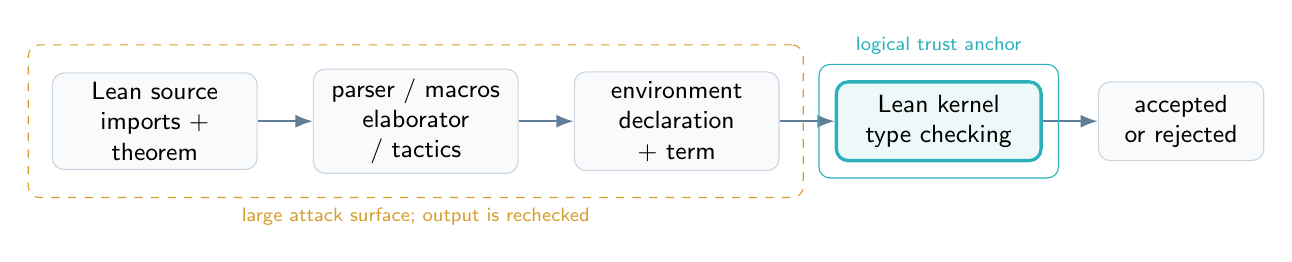
\begin{tikzpicture}[
  node distance=6mm and 7mm,
  box/.style={draw=TFLine,rounded corners=1.5mm,fill=TFPaper,minimum height=10mm,
              text width=23mm,align=center,font=\sffamily\small,inner xsep=1.5mm},
  trusted/.style={box,draw=TFCyan,line width=1.2pt,fill=TFMint!48},
  arr/.style={-{Latex[length=2.2mm]},line width=0.7pt,draw=TFMuted}
]
\node[box] (source) {Lean source\\imports + theorem};
\node[box,right=of source] (elab) {parser / macros\\elaborator / tactics};
\node[box,right=of elab] (term) {environment\\declaration + term};
\node[trusted,right=of term] (kernel) {Lean kernel\\type checking};
\node[box,right=of kernel,text width=18mm] (result) {accepted\\or rejected};
\draw[arr] (source) -- (elab);
\draw[arr] (elab) -- (term);
\draw[arr] (term) -- (kernel);
\draw[arr] (kernel) -- (result);
\node[draw=TFGold,dashed,rounded corners,fit=(source)(elab)(term),inner sep=3mm,
      label={[font=\sffamily\scriptsize,text=TFGold]below:large attack surface; output is rechecked}] {};
\node[draw=TFCyan,rounded corners,fit=(kernel),inner sep=2mm,
      label={[font=\sffamily\scriptsize,text=TFCyan]above:logical trust anchor}] {};
\end{tikzpicture}
\caption{L1 における生成経路と論理的 trust boundary}
\label{fig:trust-boundary}
\end{figure}

図\ref{fig:trust-boundary}は elaborator や tactic が無関係だという意味ではない。それらの bug は crash、
resource exhaustion、誤った error、意図しない term の生成を起こしうる。ただし、kernel が健全であり、
不正な axiom や定数を環境へ導入していない限り、誤った型の term を proof として通すことはできない。
L1 はこの構造を利用しつつ、環境の作り方と axiom を明示的に policy の対象にする。

\subsection{trusted computing base}

L1 の trusted computing base (TCB) は ``kernel binary だけ'' ではない。現実の再検証では、次が結果を
左右するため、certificate はそれらを識別しなければならない。

{\small
\begin{tabularx}{0.96\linewidth}{L{37mm}YY}
\toprule
\textbf{構成要素} & \textbf{L1 での役割} & \textbf{拘束方法} \\
\midrule
Lean kernel / runtime & declaration の型検査を実行 & release、commit、binary / image digest \\
import 済み environment & 定数、theorem、axiom を供給 & lockfile、module set、dependency digest \\
Mathlib と追加 package & 大規模な既存 theorem 群 & exact revision と package manifest \\
judge wrapper & target を構成し検査命令を実行 & wrapper version と artifact hash \\
axiom analyzer & 使用 axiom の閉包を報告 & tool version、生出力、strict parser \\
certificate encoder & field を canonicalize して署名対象化 & schema version、canonicalization version \\
\bottomrule
\end{tabularx}}

OS、container runtime、CPU は論理規則そのものではないが、replay の再現性と supply-chain integrity に
関わる。したがって platform image digest、architecture、runner identity も operational metadata として残す。

\subsection{公理に相対的な受理}

Kernel acceptance は「公理を一切使わない」を意味しない。Lean environment に declaration として存在する
axiom は、型を持つ定数として proof term から参照できる\cite{leanaxioms}。よって、
\(\Delta \vdash t : T\) は environment \(\Delta\) に相対的な judgment である。

\begin{warningbox}{重要な非同値}
\[\text{kernel accepted} \quad\not\Rightarrow\quad \text{axiom-policy compliant}.\]
\code{sorry}、custom axiom、classical choice、quotient 関連原理などの扱いは policy に依存する。
L1 certificate は kernel status と policy status を別々に記録し、両方が PASS の場合だけ
operational acceptance を発行する。
\end{warningbox}

\section{L1 acceptance の形式仕様}

\subsection{入力と judgment}

L1 判定の入力 tuple を
\[
  I=(C,A,E,q,P,\Gamma,R,X)
\]
とする。\(C\) は trusted Challenge artifact、\(A\) は exact artifact、\(E\) は environment descriptor、\(q\) は target declaration、
\(P\) は primitive axiom / namespace policy、\(\Gamma\) は certificate registry checkpoint、
\(R\) は resource envelope、\(X\) は dispatch 前の immutable JobExpectation である。Hostile builder は \(A\) を
\(E\) 内で処理し proof export \(x\) を生成するが、その process 内の \(\Delta,T,t\) を authority としない。

Verifier domain の checker judgment は次である。
\[
  V(x,E,q)=\pass \quad\Longleftrightarrow\quad
  \operatorname{LeanChecker}(x)=\pass\land\operatorname{IndependentChecker}(x)=\pass
\]

TheoremForces の operational L1 acceptance は、より強い合成 predicate とする。
\begin{align*}
L1(I)=\pass \Longleftrightarrow{}&
  \operatorname{ChallengeMatch}(C,q) \land
  \operatorname{ArtifactMatch}(A) \land
  \operatorname{EnvironmentMatch}(E) \\
 &\land\operatorname{ExpectationMatch}(X) \land
  \operatorname{Comparator}(C,q)=\pass \\
 &\land\operatorname{TargetBound}(q,x) \land
  \operatorname{UserTargetCount}(A)=1 \\
 &\land V(x,E,q)=\pass \\
 &\land\operatorname{PrimitiveAxiomPolicy}(x,E,P)=\pass \\
 &\land\operatorname{CertifiedDependencies}(x,E,\Gamma)=\pass \\
 &\land\operatorname{ResourceOutcome}(R)=\operatorname{completed} \\
 &\land\operatorname{EvidenceComplete}(I) \\
 &\land\operatorname{DurableAndLogIntegrated}(I).
\end{align*}

\begin{specbox}{Normative rule L1-1: conjunctive acceptance}
Issuer は上記 predicate の全 conjunct を機械的に確認した場合にのみ \code{l1.status = "accepted"}
を発行しなければならない。部分成功を accepted と表現してはならない。個々の sub-status は保持する。
\end{specbox}

\subsection{artifact identity}

Artifact は proof body だけではなく、判定に入力された完全な byte sequence である。最低限、次を含む。

\begin{itemize}
  \item import list、namespace、variables、statement、proof body を含む生成済み Lean file、
  \item judge が追加する wrapper / prelude の version と exact bytes、
  \item package manifest、lockfile、Lake configuration、追加 source files、
  \item source tree manifest（path、size、content hash）と root hash。
\end{itemize}

Unicode normalization、改行変換、末尾空白削除を暗黙に行ってはならない。canonical representation を作る
場合も、raw bytes の hash を必ず残す。UI に表示した reconstruction ではなく judge が読んだ bytes が基準である。

\subsection{environment identity}

Environment descriptor は、人が読む version label と機械が検証する immutable identity を分ける。

{\small
\begin{tabularx}{0.96\linewidth}{L{39mm}Y L{29mm}}
\toprule
\textbf{field} & \textbf{意味} & \textbf{要件} \\
\midrule
\code{lean.version}, \code{lean.commit} & compiler / kernel source identity & MUST \\
\code{mathlib.commit} & Mathlib revision & MUST if imported \\
\code{manifest.sha256} & full dependency resolution & MUST \\
\code{image.digest} & executable filesystem image & MUST for hosted run \\
\code{architecture} & CPU / OS execution target & MUST \\
\code{imports} & target file の import list & MUST \\
\code{environment.epoch} & platform policy 上の immutable epoch & MUST \\
\bottomrule
\end{tabularx}}

``Lean 4'' や ``latest Mathlib'' は L1 identity として不十分である。tag が movable でなくても、transitive
dependency と build option を復元できなければ replay 可能とはいえない。

\subsection{target binding}

L1 の原子単位を \term{one attempt = one theorem} とする。user payload は top-level の
\code{theorem} / \code{lemma} を厳密に一つだけ含まなければならない。複数の declaration のうち一つだけを target として
選ぶ方式は採用しない。使われない第二 theorem も \code{multiple\_target\_declarations} として拒否する。
proof 内の \code{have}、\code{let}、local function は単一 proof term に閉じるため許可できるが、再利用する補助定理は
別 attempt で certificate 化しなければならない。server-generated wrapper declaration は count から除外し、その exact
bytes と template version を artifact に拘束する。

judge は唯一の target の fully qualified name、expected type hash、source span、declaration kind を記録する。

\begin{specbox}{Normative rule L1-2: single user target}
Issuer は user-supplied top-level target declaration 数が一つであり、その selector が environment 内でただ一つの
declaration に解決されることを確認しなければならない。0 件、2 件以上、名前の shadowing、expected type の不一致を
受理してはならない。
\end{specbox}

可能なら judge wrapper が新しい namespace と衝突しない generated identifier を用意し、対象 statement と
proof body を直接結合する。既存 theorem と同名の declaration を偶然参照して通過する経路をなくす。

\subsection{複数定理 UX は L1 の外に置く}

UI / API は複数 theorem の一括入力を提供してよい。ただし batch orchestrator が入力を $N$ 個の独立 artifact に分け、
$N$ 個の L1 attempt、resource envelope、result、certificate を生成する。batch / collection manifest は結果の集約であり、
L1 certificate ではない。部分成功を許容し、失敗した job だけを retry する。この境界により、一つの theorem の失敗で
別 theorem の historical acceptance が曖昧にならず、cache、quota、citation、dependency edge も theorem 単位になる。

\begin{specbox}{Normative rule L1-3: no atomic multi-target acceptance}
Issuer は複数 theorem を一つの \code{l1.status = "accepted"} に畳み込んではならない。collection の status は
各 child attempt への参照と集計値だけを持ち、独自の kernel acceptance を主張しない。
\end{specbox}

\section{axiom policy}

\subsection{三段階の判定}

axiom analyzer は、kernel checking 後に target の transitive dependency closure を調べ、
\term{primitive assumptions} と \term{certificate-backed assumptions} に分離する。前者だけを
\term{allowed}、\term{denied}、\term{unknown} に分類し、unknown は fail-closed とする。後者は名前ではなく
certificate registry によって検証する。

\begin{enumerate}
  \item target declaration から参照定数を再帰的に列挙する。
  \item opaque / theorem boundary を含め、primitive axiom 集合と certificate dependency 集合を得る。
  \item primitive assumption は canonical axiom identifier と environment-local identifier を対応付ける。
  \item certificate assumption は registry object、type hash、logical environment digest と対応付ける。
  \item primitive policy と certificate chain の両方が PASS のときだけ operational policy status を PASS にする。
\end{enumerate}

Lean の \code{\#print axioms} は debugging 用の補助 evidence として保存してよいが、L1 acceptance authority に
してはならない。Pinned proof exporter と二つの checker が proof export から structured transitive closure を再計算し、
human-oriented stdout の parse failure、format drift、truncation は indeterminate とする\cite{leanvalidate}。

\subsection{certificate-backed assumption}

一度 L1 accepted された theorem は、downstream elaboration cache として server-generated な opaque / axiom stub を
利用してよい。ただし stub build は certificate assumptions に相対的な結果であり、L1 issuance の checker path は
全 upstream proof export を topological order で再検査する。概念的 cache は次の形である。

\begin{lstlisting}
namespace TheoremForces.Certified
-- Generated only after resolving certificate sha256:<c>.
axiom c_<certificate_hash> : <exact certified statement>
end TheoremForces.Certified
\end{lstlisting}

これは「user axiom を許可する」ことではない。namespace の文字列一致では受理せず、resolver が certificate hash から
生成した module hash、stub の canonical type hash、発行時の logical environment digest を照合する。user-defined axiom、
同名 declaration、改変された stub は拒否する。accepted theorem の historical artifact は保持し、full verifier は
certificate chain を再帰的に replay する。一つでも certified dependency があれば UI / API / CLI は axiom-free または
unconditional proof と表示しない。

primitive axiom 集合を $P_E(t)$、certificate-backed dependency 集合を $C_E(t)$ とする。certificate import の条件は

\[
  \forall c\in C_E(t),\quad
  \operatorname{ActiveAtIssue}(c,\Gamma_{issue})\land
  \operatorname{TypeHashMatch}(c)\land
  \operatorname{LogicalEnv}(c)=E,
\]

かつ $C_E(t)$ の transitive graph が acyclic で、全 upstream certificate に同じ条件が成り立つことである。
発行時 validity と current status を分離する。Dependency が invalidated / retracted-by-policy になった場合、downstream certificate を削除せず tainted event を追加し、
再発行を停止して影響 closure を再検証する。

\begin{specbox}{Normative rule L1-4: same logical environment}
Certificate-backed assumption は、Lean version、Mathlib / package manifest、primitive axiom policy、wrapper / analyzer rule を
含む \code{logical\_environment\_digest} が importing attempt と一致する場合にだけ使用できる。human-readable label や
registry namespace の一致だけで cross-environment import を許可してはならない。
\end{specbox}

\subsection{推奨 policy profile}

\begin{tabularx}{\linewidth}{L{34mm}L{30mm}Y}
\toprule
\textbf{category} & \textbf{default} & \textbf{理由と表示} \\
\midrule
\code{sorryAx} / synthetic sorry & deny & 未完了証明を完全な proof と表示しない \\
user-defined axiom & deny & 明示的 review なしの仮定導入を防ぐ \\
Lean / Mathlib standard axioms & explicit allowlist & profile と environment ごとに名前を固定 \\
unrecognized declaration & unknown $\rightarrow$ deny & analyzer / package drift を安全側で扱う \\
unsafe implementation detail & separate operational check & 論理公理と runtime risk を混同しない \\
\bottomrule
\end{tabularx}

``axiom-free'' という label は、使用集合が空であることを再検証可能に示せる場合だけ使う。
標準的な古典論理の原理を許可する profile は、単に ``L1 accepted'' とし、実際の axiom set を併記する。

\subsection{policy versioning}

Axiom policy は immutable object として content-addressed storage に置く。certificate は
\code{policy.id}、\code{policy.sha256}、判定時の classification を持つ。後日 policy が変わっても、historical
record は変えず、新 policy による再評価 event を追加する。これにより ``当時は受理、現在 profile では拒否'' を
正確に表現できる。

accepted theorem を追加するたびに primitive axiom policy を更新してはならない。logical base epoch $E$ と primitive
policy $P$ は低頻度で versioning し、same-$E$ certificate の集合は append-only registry checkpoint
$\Gamma_0,\Gamma_1,\ldots$ として高頻度に更新する。import は exact certificate hash を指すため、checkpoint が進んでも
既存 certificate の意味は変わらない。別 $E$ へ移すときは migration replay と新 certificate が必要である。

\begin{decisionbox}{頻繁に変わるのは「公理 policy」ではなく registry root}
新しく accepted された命題は primitive allowlist に追加しない。certificate-backed assumption として registry に追記する。
したがって standard axiom profile の version は安定し、頻繁な更新は content-addressed checkpoint root に局所化される。
\end{decisionbox}

\section{判定 pipeline と状態機械}

\subsection{fail-closed pipeline}

\begin{figure}[htbp]
\centering
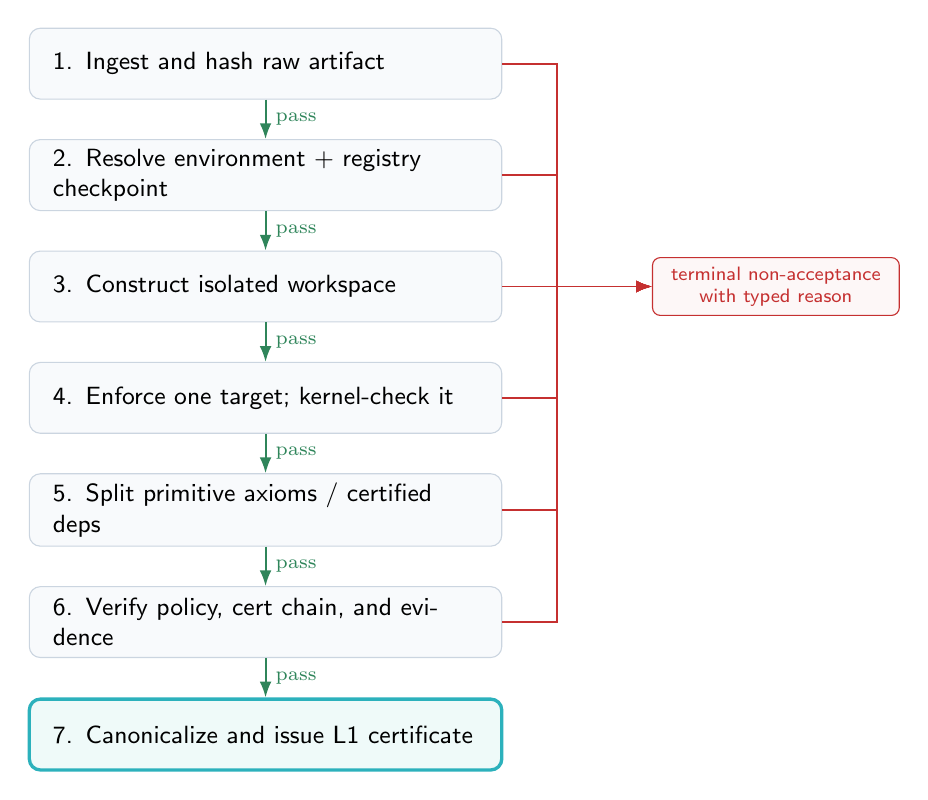
\begin{tikzpicture}[
  node distance=5mm,
  pipestep/.style={draw=TFLine,rounded corners=1.4mm,fill=TFPaper,minimum height=9mm,
               text width=54mm,align=left,font=\sffamily\small,inner xsep=3mm},
  ok/.style={-{Latex[length=2mm]},draw=TFGreen,line width=0.7pt},
  bad/.style={-{Latex[length=2mm]},draw=TFRed,line width=0.7pt},
  failnode/.style={draw=TFRed,rounded corners=1mm,fill=TFRed!4,text=TFRed,
                   font=\sffamily\scriptsize,align=center,text width=29mm}
]
\node[pipestep] (s1) {1. Ingest and hash raw artifact};
\node[pipestep,below=of s1] (s2) {2. Resolve environment + registry checkpoint};
\node[pipestep,below=of s2] (s3) {3. Construct isolated workspace};
\node[pipestep,below=of s3] (s4) {4. Enforce one target; kernel-check it};
\node[pipestep,below=of s4] (s5) {5. Split primitive axioms / certified deps};
\node[pipestep,below=of s5] (s6) {6. Verify policy, cert chain, and evidence};
\node[pipestep,below=of s6,draw=TFCyan,line width=1.2pt,fill=TFMint!42] (s7) {7. Canonicalize and issue L1 certificate};
\foreach \a/\b in {s1/s2,s2/s3,s3/s4,s4/s5,s5/s6,s6/s7}{\draw[ok] (\a) -- node[right,font=\scriptsize,text=TFGreen]{pass} (\b);}
\node[failnode,right=19mm of s3] (f) {terminal non-acceptance\\with typed reason};
\foreach \a in {s1,s2,s3,s4,s5,s6}{\draw[bad] (\a.east) -- ++(7mm,0) |- (f.west);}
\end{tikzpicture}
\caption{L1 judge の一方向 pipeline。失敗後に受理経路へ復帰しない。}
\label{fig:pipeline}
\end{figure}

各 stage は input / output digest、開始・終了時刻、runner identity、typed result を記録する。
retry は同じ run の書換えではなく新しい attempt とし、certificate が参照する attempt を一意にする。

\subsection{結果 taxonomy}

\begin{longtable}{L{39mm}L{29mm}L{75mm}}
\toprule
\textbf{result code} & \textbf{L1} & \textbf{意味} \\
\midrule
\endfirsthead
\toprule
\textbf{result code} & \textbf{L1} & \textbf{意味} \\
\midrule
\endhead
\code{accepted} & accepted & kernel と全 operational predicate が PASS \\
\code{parse\_or\_}\newline\code{elaboration\_failure} & not accepted & source から target declaration を構成できない \\
\code{kernel\_or\_type\_error} & not accepted & target term が期待する type を持たない \\
\code{multiple\_target\_}
\newline\code{declarations} & not accepted & user payload に top-level theorem / lemma が 2 件以上 \\
\code{axiom\_policy\_rejection} & not accepted & deny または unknown axiom を検出 \\
\code{certificate\_}\newline\code{dependency\_invalid} & not accepted & certificate、type hash、status、closure が不正 \\
\code{certificate\_}\newline\code{environment\_}\newline\code{mismatch} & not accepted & dependency と importing attempt の logical environment が不一致 \\
\code{certificate\_}\newline\code{dependency\_cycle} & not accepted & certificate dependency graph に cycle を検出 \\
\code{target\_mismatch} & not accepted & name、type hash、declaration identity が不一致 \\
\code{artifact\_mismatch} & not accepted & judge input と certificate 対象の bytes が不一致 \\
\code{resource\_exhausted} & indeterminate & timeout、memory、disk、process quota 超過 \\
\code{infrastructure\_error} & indeterminate & image、storage、scheduler、network 等の障害 \\
\code{evidence\_incomplete} & indeterminate & axiom report、manifest、log 等の必須証拠が欠落 \\
\bottomrule
\end{longtable}

\term{not accepted} は反例や数学的偽を意味しない。\term{indeterminate} は再試行可能だが、accepted と表示しては
ならない。UI、API、export、analytics は同じ taxonomy を使い、HTTP status や自由文 log から意味を再推定しない。

\subsection{resource envelope}

CPU、wall time、memory、file size、process count、output bytes に上限を設ける。上限は certificate に記録し、
超過を proof failure と区別する。resource policy の目的は logical soundness そのものではなく、公平性、可用性、
abuse containment である。sandbox が破られても kernel acceptance record を偽造できないよう、証明書 signing と
public ledger ingestion は judge process から分離する。

\section{L1 certificate schema}

\subsection{必須 field}

L1 certificate は self-contained な metadata と content-addressed artifact への参照を持つ。最低限の schema を
表\ref{tab:schema}に示す。表中の CertificateCore field path は \code{core.} prefix を省略し、
\code{issuance\_attestation} と \code{log\_receipt} だけは envelope root からの path を記す。

\begin{longtable}{@{}L{44mm}L{27mm}L{72mm}@{}}
\caption{L1 certificate の normative field}\label{tab:schema}\\
\toprule
\textbf{field} & \textbf{type} & \textbf{requirement} \\
\midrule
\endfirsthead
\toprule
\textbf{field} & \textbf{type} & \textbf{requirement} \\
\midrule
\endhead
\code{schema}, \code{certificate\_id} & string & core schema version と globally unique ID \\
\code{attempt\_id},\newline\code{target.challenge\_}\newline
\code{artifact\_sha256} & string / digest & immutable attempt と organizer-controlled Challenge \\
\code{artifact.upload\_raw\_}\newline\code{sha256} & digest & transport で受け取った exact bytes \\
\code{artifact.entrypoint\_raw\_}\newline\code{sha256} & digest & decoded Lean entrypoint exact bytes \\
\code{artifact.manifest\_sha256} & digest & canonical path / size / mode / file hash manifest \\
\code{artifact.bundle\_root\_}\newline\code{sha256} & digest & domain-separated canonical manifest root \\
\code{artifact.generated\_}\newline\code{source\_sha256} & digest & builder が実際に読んだ generated source \\
\code{environment.epoch} & string & immutable platform environment \\
\code{environment.}\newline\code{logical\_digest} & digest & Lean、packages、primitive policy、wrapper rule の identity \\
\code{environment.}\newline\code{manifest\_sha256} & digest & Lean、packages、options の完全 manifest \\
\code{environment.image\_digest} & digest & hosted execution image \\
\code{target.fqname} & string & fully qualified declaration name \\
\code{target.user\_}\newline\code{declaration\_count} & integer & MUST equal 1 \\
\code{target.declaration\_kind} & enum & MUST equal theorem \\
\code{target.universe\_}\newline\code{parameters\_format /}\newline
\code{universe\_parameters\_}\newline\code{sha256} & string / digest & versioned universe parameters \\
\code{target.type\_format / type\_sha256} & string / digest & versioned target type \\
\code{target.value\_format / value\_sha256} & string / digest & versioned target value \\
\code{target.proof\_export\_}\newline\code{format / proof\_export\_}\newline
\code{sha256} & string / digest & versioned proof export \\
\code{comparator.status} & enum & trusted Challenge equality PASS / non-PASS \\
\code{checkers.items} & array & Lean checker と independent checker の identity / result / evidence digest \\
\code{axioms.primitive\_items} & array & primitive axiom set と classification \\
\code{axioms.raw\_report\_sha256} & digest & analyzer の raw evidence \\
\code{certified\_dependencies.}\newline\code{items} & array & cert / type hash、constant、direct / transitive edge \\
\code{certified\_dependencies.}\newline\code{registry\_checkpoint} & digest & 判定に使った event-prefix checkpoint \\
\code{certified\_dependencies.}\newline\code{closure\_sha256} & digest & acyclic dependency closure の identity \\
\code{policy.id}, \code{policy.sha256} & string / digest & immutable policy identity \\
\code{run.outcome} & enum & accepted core では MUST equal completed \\
\code{run.limits / usage} & object & CPU、wall、RSS、PID、file、disk、inode、output、network の limit と actual \\
\code{run.stdout\_sha256 /}\newline\code{run.stderr\_sha256} & digests & 完全 log への content address と truncation flag \\
\code{l1.status}, \code{l1.reason} & enum & accepted と typed decision reason \\
\code{issuance\_attestation.}\newline\code{payload.core\_sha256} & digest & domain-separated JCS CertificateCore digest \\
\code{issuance\_attestation.}\newline\code{payload / signature} & objects & core / expectation / result / verifier quorum と Ed25519 envelope \\
\code{log\_receipt} & object & cumulative inclusion / consistency / checkpoint / witness evidence \\
\bottomrule
\end{longtable}

\subsection{canonical JSON 例}

次は三層 topology の縮約例である。掲載した field names とその object topology は normative schema に一致するが、
紙幅のため required field の一部を省略している。この紙面例自体を test vector にせず、repository の完全 fixture を
JCS / schema / signature / Merkle test に使う。

\begin{lstlisting}[language=JSON,basicstyle=\ttfamily\scriptsize]
{
  "schema": "theoremforces.l1-certificate/2",
  "core": {
    "schema": "theoremforces.l1-core/2",
    "certificate_id": "tf-l1-01JEXAMPLE",
    "attempt_id": "01JATTEMPT",
    "issued_at": "2026-08-09T12:00:00Z",
    "event_sequence": 42,
    "artifact": {
      "upload_raw_sha256": "sha256:...",
      "upload_raw_uri": "cas://sha256/...",
      "entrypoint_raw_sha256": "sha256:...",
      "entrypoint_raw_uri": "cas://sha256/...",
      "manifest_sha256": "sha256:...",
      "manifest_uri": "cas://sha256/...",
      "bundle_root_sha256": "sha256:...",
      "generated_source_sha256": "sha256:...",
      "generated_source_uri": "cas://sha256/...",
      "proof_export_sha256": "sha256:...",
      "proof_export_uri": "cas://sha256/..."
    },
    "environment": {
      "logical_digest": "sha256:...",
      "manifest_sha256": "sha256:...",
      "image_digest": "sha256:...",
      "architecture": "linux/amd64"
    },
    "target": {
      "challenge_id": "tf-challenge-01JEXAMPLE",
      "challenge_artifact_sha256": "sha256:...",
      "challenge_artifact_uri": "cas://sha256/...",
      "fqname": "TheoremForces.Attempt.solution_target",
      "user_declaration_count": 1,
      "declaration_kind": "theorem",
      "type_sha256": "sha256:...",
      "value_sha256": "sha256:...",
      "proof_export_sha256": "sha256:..."
    },
    "certified_dependencies": {
      "status": "pass",
      "registry_checkpoint": "sha256:...",
      "items": [],
      "closure_sha256": "sha256:..."
    },
    "axioms": {
      "status": "pass",
      "policy_sha256": "sha256:...",
      "primitive_items": [],
      "closure_sha256": "sha256:..."
    },
    "comparator": {"status": "pass", "evidence_sha256": "sha256:..."},
    "checkers": {"status": "pass", "items": [
      {"role": "lean_checker", "status": "pass"},
      {"role": "independent_checker", "status": "pass"}
    ]},
    "run": {"outcome": "completed", "structured_result_count": 1},
    "l1": {"status": "accepted", "reason": "all_predicates_passed"}
  },
  "issuance_attestation": {
    "schema": "theoremforces.l1-issuance-envelope/1",
    "payload": {
      "schema": "theoremforces.l1-issuance/1",
      "core_sha256": "sha256:...",
      "job_expectation_sha256": "sha256:...",
      "result_attestation_sha256": "sha256:...",
      "issuer": {"key_id": "tf-issuer-2026-01", "algorithm": "Ed25519"},
      "issued_at": "2026-08-09T12:00:00Z"
    },
    "signature": "..."
  },
  "log_receipt": {
    "schema": "theoremforces.l1-log-receipt/2",
    "core_sha256": "sha256:...",
    "issuance_sha256": "sha256:...",
    "leaf_hash": "sha256:...",
    "tree_size": 42,
    "leaf_index": 41,
    "inclusion_path": [],
    "checkpoint": {
      "schema": "theoremforces.l1-log-checkpoint-envelope/2",
      "payload": {
        "schema": "theoremforces.l1-log-checkpoint/2",
        "log_id": "tf-log-v2",
        "algorithm": "rfc6962-sha256",
        "tree_size": 42,
        "root_sha256": "sha256:...",
        "maximum_merge_delay_ms": 300000
      },
      "signature": "..."
    },
    "consistency": {
      "old_tree_size": 41,
      "old_root_sha256": "sha256:...",
      "consistency_path": []
    },
    "witness_receipts": [
      {"schema": "theoremforces.l1-witness-envelope/2",
       "payload": {"witness": {"witness_id": "witness-a"}}, "signature": "..."},
      {"schema": "theoremforces.l1-witness-envelope/2",
       "payload": {"witness": {"witness_id": "witness-b"}}, "signature": "..."}
    ]
  }
}
\end{lstlisting}

\subsection{署名対象と transparency}

Ed25519 signature message は前節で定義した $m_I$、すなわち
\code{theoremforces.l1.signature.v2} domain、NUL separator、
\code{issuance\_attestation.payload} の JCS bytes の順の連結とする。Signature 自身、LogReceipt、witness は
signed payload の外側であり自己参照しない。Private signing key は judge / builder container に置かず、separate issuer
service が verifier quorum と全 predicate を再確認した後だけ使用する。公開 key の validity、rotation、revocation を
append-only event log に残す。署名は issuer を認証するが、checker quorum と artifact replay の代替ではない。

\section{独立 verifier}

\subsection{三つの検証 mode}

\begin{tabularx}{\linewidth}{L{34mm}L{33mm}Y}
\toprule
\textbf{mode} & \textbf{確認範囲} & \textbf{用途} \\
\midrule
Metadata verification & strict schema、core / issuance digest、signature、log inclusion / consistency / witnesses & non-executing citation / UI 検査 \\
Historical replay & mandatory sandbox + certificate と同じ environment & 元の L1 claim の独立再現 \\
Migration replay & 新しい environment / policy & current compatibility の追加評価 \\
\bottomrule
\end{tabularx}

Historical replay と migration replay を混同しない。後者が失敗しても historical acceptance は消えず、
\code{reverification} event に結果を追加する。

\subsection{verifier algorithm}

\begin{lstlisting}[language={},basicstyle=\ttfamily\scriptsize]
verify_l1(certificate C):
  validate_schema_strict(C)
  core_sha256 = core_digest(C.core)
  issuance_sha256 = issuance_digest(C.issuance_attestation.payload)
  require C.issuance_attestation.payload.core_sha256 == core_sha256
  verify_ed25519_envelope(C.issuance_attestation)
  verify_key_valid_at_issuance_checkpoint(C.issuance_attestation)
  fetch artifact_manifest, environment_manifest, policy, evidence
  require every fetched object's digest equals the digest in C
  require canonical artifact manifest and bundle root match C.core
  require immutable JobExpectation matches signed ResultAttestation
  resolve certified dependencies at
          C.core.certified_dependencies.registry_checkpoint
  require every certificate was valid at issuance checkpoint
  report current dependency status and taint separately
  require every dependency type/value/export hash matches
  require the transitive certificate graph is acyclic
  require C.log_receipt.core_sha256 == core_sha256
  require C.log_receipt.issuance_sha256 == issuance_sha256
  verify cumulative log inclusion, consistency, checkpoint signature
  require at least two valid independent witness receipts
  require recorded Comparator and both checker receipts are PASS
  if explicit --replay:
    reconstruct only inside mandatory sandbox
    require trusted Challenge Comparator equality
    export and inspect proof outside hostile builder sandbox
    require Lean checker PASS and independent checker PASS
    require type/value/export/axiom/resource digests match C.core
  return an assurance vector, never one ambiguous VERIFIED boolean
\end{lstlisting}

verifier は network から取得した object を digest 確認前に実行しない。archive extraction の path traversal、
symlink escape、decompression bomb を拒否する。signature が正しくても artifact が取得不能なら
\term{metadata-verified / replay-unavailable} とし、full verification と表示しない。

\subsection{determinism と許容差}

Lean build の wall time や log ordering は完全には deterministic でない。L1 が一致を要求するのは、target identity、
kernel result、axiom set、入力 digest である。timestamp、runner ID、性能値は attempt-local metadata とする。
同じ入力で論理結果が分岐した場合は severity-1 integrity incident として新規発行を止める。

\section{脅威モデル}

\subsection{保護対象と攻撃者}

保護対象は、(1) accepted status の真正性、(2) artifact と environment の同一性、(3) axiom report の完全性、
(4) historical ledger の非改変性、(5) judge availability である。攻撃者として malicious submitter、侵害された
runner、誤設定された deploy、supply-chain attacker、権限を持つ insider を想定する。

\begin{longtable}{L{39mm}L{51mm}L{53mm}}
\toprule
\textbf{threat} & \textbf{attack} & \textbf{required control} \\
\midrule
\endfirsthead
\toprule
\textbf{threat} & \textbf{attack} & \textbf{required control} \\
\midrule
\endhead
Source substitution & UI 表示と judge input を差し替える & raw-byte hash、manifest、CAS、署名 binding \\
Target confusion & 別 theorem / 既存 theorem を通す & generated namespace、fqname、type hash \\
Multi-target smuggling & 第二 theorem に未監査の前提や副作用を隠す & one user target validator、batch fan-out \\
Hidden axiom & \code{sorry} や custom axiom を依存へ埋める & transitive closure、strict allowlist、raw evidence \\
Certified namespace spoof & registry にない同名 axiom / stub を作る & server-generated module、cert / type / module hash \\
Cross-epoch certificate & 異なる axiom / package 環境の theorem を流用 & logical environment digest equality、migration certificate \\
Dependency cycle / revocation & 循環で検証を逃れる、失効 theorem を継続利用 & DAG check、append-only status、downstream taint \\
Parser drift & axiom output の未知形式を空集合と読む & version pin、strict parse、unknown = reject \\
Fake callback & runner success を署名なしで ledger へ送る & authenticated channel、ledger-side predicate check \\
Image substitution & label は同じで binary を交換 & immutable digest、registry verification、attestation \\
Dependency omission & manifest 外から package を読む & offline build、read-only store、network deny \\
Resource escape & fork bomb、file / network abuse & namespace、cgroup、seccomp、quota、egress policy \\
Log truncation & error を隠し success 部分だけ保存 & complete-log digest、exit status、size-limit outcome \\
Ledger rewrite & historical failure を success に置換 & append-only events、external checkpoint、audit export \\
Key compromise & 偽 certificate を署名 & HSM / isolated signer、rotation、revocation、transparency log \\
\bottomrule
\end{longtable}

\subsection{sandbox と logical soundness の分離}

Sandbox は infrastructure を守り、他 submission との isolation を提供する。kernel checking は logical claim を
検査する。sandbox が強いことは proof の正しさを意味せず、proof が正しいことは arbitrary code execution が安全で
あることを意味しない。security documentation と judge の実装要件は、この二つの control plane を分けて扱う
\cite{tfsecurity,tfjudging}。

\subsection{residual risk}

L1 は Lean kernel 自体の soundness bug、hardware fault、compiler / runtime の supply-chain compromise を数学的に
排除しない。対策は TCB 縮小、exact version、複数 runner での再検証、公開 artifact、upstream advisory monitoring、
incident response である。高価値 certificate には異なる architecture または独立運営者による replay receipt を
追加することを SHOULD とする。

\section{reproducibility と migration}

\subsection{三つの時間軸}

Certificate の状態は一つの boolean でなく、少なくとも次の時間軸を持つ。

\begin{itemize}
  \item \term{Historical L1}: 発行時 environment / policy で accepted だったか。
  \item \term{Active replay}: platform の active environment で現在も accepted か。
  \item \term{Upstream compatibility}: 指定した新 Lean / Mathlib candidate で accepted か。
\end{itemize}

新 environment で失敗したとき、元 certificate の \code{l1.status} を書き換えてはならない。
\code{reverification\_failed} event に environment、reason、log digest を追加する。statement または proof を修正した
場合は新 artifact で新 certificate を発行し、\code{supersedes} edge で関係を示す。

\subsection{artifact retention}

Full replay のため、source bundle、manifests、policy、raw axiom report、build log、必要なら build image を保持する。
保持期間を短縮する場合、certificate は再現性 level を明示する。最低でも content digest と複数 location を持ち、
消失を静かに無視しない。ledger は公開 export と定期 checkpoint を提供し、platform 終了後も検証可能性を残す
\cite{tfledger}。

\subsection{environment epoch の lifecycle}

\begin{enumerate}
  \item candidate epoch を content-addressed manifest として作成する。
  \item golden / negative / malicious corpus を replay する。
  \item active 化前に差分 report と known breakage を公開する。
  \item old epoch を historical replay 用に read-only 保持する。
  \item certificate ごとの migration result を append-only event として追加する。
\end{enumerate}

\section{testing と observability}

\subsection{verification corpus}

Unit test だけでは L1 boundary を守れない。次の corpus を CI と production canary の両方で使う。

\begin{tabularx}{0.96\linewidth}{L{38mm}Y L{42mm}}
\toprule
\textbf{suite} & \textbf{fixture} & \textbf{expected invariant} \\
\midrule
Golden proofs & 小さな accepted theorem と実研究例 & target / axiom / digest が固定 \\
Negative proofs & type error、未定義名、false target & 決して accepted にならない \\
Axiom attacks & \code{sorryAx}、custom axiom、間接依存 & deny / unknown を確実に拒否 \\
Target attacks & shadowing、duplicate name、type drift & target mismatch \\
Target cardinality & 0 / 2+ top-level theorem、unused second theorem & exactly one or typed rejection \\
Batch facade & 3 theorem、partial failure、child retry & 3 independent attempts; no batch L1 \\
Certified imports & valid same-$E$ cert、spoof、cross-$E$、cycle、revoked cert & only valid acyclic same-$E$ chain passes \\
Artifact attacks & newline、Unicode、symlink、path traversal & exact hash または ingest rejection \\
Resource attacks & loop、huge output、memory pressure & exhausted、runner recovery \\
Schema attacks & unknown field、duplicate key、bad Unicode & strict parser rejection \\
Replay matrix & architecture / clean host / independent operator & logical output 一致 \\
\bottomrule
\end{tabularx}

Property test は canonical JSON の一意性、manifest path normalization、hash stability、status state machine の
不正遷移を対象にする。production deploy は corpus の全 gate を通過しなければならない。

\subsection{integrity SLO と運用 metric}

可用性より integrity を優先する。推奨する初期 SLO / invariant は次である。

\begin{itemize}
  \item accepted certificate の必須 digest / target / axiom report 完備率: \term{100\%}、
  \item accepted certificate に対する corpus-based false acceptance: \term{0}、
  \item 同一 attempt が複数の terminal state を持つ件数: \term{0}、
  \item daily sampled historical replay の一致率: \term{100\%}、
  \item infrastructure error、resource exhaustion、queue latency は別 metric として公開、
  \item artifact retrieval failure と replay unavailable を成功率から除外せず可視化。
\end{itemize}

一件でも false acceptance または artifact mismatch が確認されたら、L1 発行を停止し、key / environment / affected
certificate 範囲を調査する。過去 event は削除せず incident marker と再検証結果を追加する。

\section{実装 roadmap}

\subsection{Phase 0: claim freeze と fixture（0--30日）}

\begin{itemize}
  \item 本書の predicate、taxonomy、schema を versioned specification として固定する。
  \item one user target validator と generated namespace を実装し、target count と type hash を記録する。
  \item multi-theorem request を独立 child job に分解する batch boundary と fixture を固定する。
  \item primitive axiom と certificate-backed dependency を schema / analyzer / UI で分離する。
  \item raw artifact bundle と environment manifest の content hashing を実装する。
  \item \code{sorryAx}、custom axiom、unknown parser output の negative fixture を追加する。
  \item UI / API の ``accepted'' 表示経路を棚卸しし、唯一の合成 predicate に統合する。
\end{itemize}

\begin{decisionbox}{Gate A}
Golden / negative / axiom / target corpus が CI で 100\% deterministic に通り、accepted を生成できる code path が
ledger-side L1 predicate の一つだけであること。未達なら外部向け certificate claim を拡張しない。
\end{decisionbox}

\subsection{Phase 1: certificate と replay（31--60日）}

\begin{itemize}
  \item L1 schema、canonical encoder、signature、public key discovery を実装する。
  \item same-environment certificate registry、content-addressed stub generator、checkpoint root を実装する。
  \item source / environment / policy / evidence を CAS に置き、certificate から取得可能にする。
  \item independent verifier CLI を別 package として作り、metadata / historical replay を提供する。
  \item retry を append-only attempt に変更し、terminal state の上書きを禁止する。
  \item staging certificate を clean host と第二 architecture で再検証する。
  \item valid / spoofed / cross-epoch / cyclic / revoked certificate import corpus を通す。
\end{itemize}

\begin{decisionbox}{Gate B}
無作為抽出した staging certificate を clean host で artifact から再構成でき、target identity、kernel result、axiom
set が全件一致すること。取得不能、手作業修正、moving tag 依存が一件でもあれば未達とする。
\end{decisionbox}

\subsection{Phase 2: production hardening（61--90日）}

\begin{itemize}
  \item signer を runner から分離し、key rotation / revocation / transparency checkpoint を導入する。
  \item sandbox profile、egress deny、quota、archive extraction 防御を adversarial test する。
  \item sampled daily replay、integrity alert、issuance kill switch、incident playbook を運用する。
  \item environment migration の candidate corpus と append-only reverification event を実装する。
  \item certificate invalidation の downstream taint propagation と issuance kill switch を drill する。
  \item atomic persistence design を ADR で固定し、certificate / economy / ledger / bounty の crash / concurrency corpus を全件通す。
  \item public L1 export と verifier documentation を公開し、外部 operator の replay receipt を受け付ける。
\end{itemize}

\begin{decisionbox}{Gate C}
30 日間、必須 evidence 完備率 100\%、sampled replay 一致率 100\%、false acceptance 0 を維持し、
kill switch と key revocation drill を完了すること。この 30 日 clock は L1-ATOM-001 の crash / concurrency corpus が
100\% 合格した後にのみ開始する。これを L1 production readiness の最低条件とする。
\end{decisionbox}

\subsection{ownership}

\begin{tabularx}{\linewidth}{L{37mm}L{37mm}Y}
\toprule
\textbf{workstream} & \textbf{accountable role} & \textbf{review separation} \\
\midrule
Kernel / target wrapper & judge maintainer & adversarial fixture reviewer \\
Axiom analyzer / policy & formalization maintainer & policy approver \\
Artifact / environment CAS & platform maintainer & reproducibility operator \\
Certificate / ledger / signer & security owner & key custodian + audit reviewer \\
Verifier CLI & independent tooling owner & must not reuse issuer trust decisions blindly \\
Incident response & service owner & public post-incident approver \\
\bottomrule
\end{tabularx}

小規模 team でも role を文書上分け、同じ人が実装する場合は時間を分けた review と公開 fixture で補う。

\section{決定事項と非規範的 research questions}

\subsection{本仕様で固定する決定}

\begin{enumerate}
  \item L1 は kernel acceptance と operational predicate の conjunction とする。
  \item Kernel status と axiom-policy status を別 field とする。
  \item exact raw artifact、environment、target type を digest で拘束する。
  \item 一つの L1 attempt は user-supplied top-level theorem を一つだけ持つ。
  \item multi-theorem UX は L1 外部で独立 child attempt へ fan-out する。
  \item accepted theorem の再利用は primitive allowlist ではなく、same-environment certificate registry で管理する。
  \item logical epoch / primitive policy と append-only registry checkpoint を別に versioning する。
  \item timeout、infrastructure error、unknown axiom / parser は fail-closed とする。
  \item retry、migration、revocation は append-only event とし、historical result を上書きしない。
  \item Certificate / economy / ledger / bounty の multi-row mutation は proven atomic boundary に置き、未達時は全経路を fail-closed にする。
  \item platform signature を replay の代替にしない。
  \item target identity は pinned versioned kernel declaration / proof export encoding とし、pretty-printer を使わない。
  \item canonical JSON は RFC 8785 JCS + I-JSON、signature は Ed25519、三層 envelope とする。
  \item axiom closure は proof export から checker domain で再計算し、stdout parser を authority にしない。
  \item registry event / checkpoint と replay objects は certificate lifetime 中保持し、two-witness cumulative log を使う。
\end{enumerate}

\subsection{Accepted の意味を変えない research questions}

\begin{itemize}
  \item standard axiom profile を単一にするか、constructive / classical など複数 profile を持つか。
  \item 必須の two-witness quorum を超えて、どの operator / jurisdiction に mirror を増やすか。
  \item Full-chain replay の latency を下げる content-addressed cache を、trust decision と分離してどう運用するか。
  \item Stable export format の次 version を Lean upstream とどう共同設計するか。
  \item Current taint と historical validity の差を non-expert UI でどう説明するか。
\end{itemize}

これらは Gate 0 の決定を弱めてはならない。Accepted の意味を変更する proposal は research question のまま実装せず、
new schema / policy version、ADR、golden vectors、migration plan、Gate A--C の再実行を必要とする。

\section{結論}

L1 の価値は、強く聞こえる label ではなく、主張を小さくし、入力と環境を固定し、失敗を隠さず、誰でも replay
できることにある。Lean kernel は formal derivability の強い trust anchor だが、hostile input では Comparator、
proof export、official checker、independent checker と組み合わせる必要がある。その事実を公共の certificate に
変えるには artifact、target、axiom、resource、ledger の境界を正確に設計する必要がある。

TheoremForces は、すべての数学的評価を L1 に押し込めるべきではない。L1 は「この一つの exact theorem が、この exact
environment、primitive axiom policy、certificate dependency chain のもとで受理された」という狭い事実を堅牢に残す。
その上に provenance、migration、
intent review、curation を積むことで、AI 時代の形式数学に必要な検証可能性を段階的に構築できる。

\begin{principlebox}{最終原則}
No artifact, no L1. No exact environment, no L1. Not exactly one target, no L1.
No primitive / certified dependency evidence, no L1. No Comparator and checker quorum, no L1.
No independent replay path, no durable trust.
\end{principlebox}

\appendix
\section{minimal judge wrapper 例}

次の例は target binding の考え方を示すだけであり、production sandbox や analyzer の完全実装ではない。

\begin{lstlisting}
import Mathlib
import TheoremForces.Certified.Dep_<certificate_hash>

namespace TheoremForces.Submission.Generated_01JEXAMPLE

-- The exact statement and proof body are inserted as raw artifact content.
-- This is the only user-supplied top-level theorem in the attempt.
theorem solution_target (n : Nat) : n + 0 = n := by
  simp

-- The judge resolves this fully qualified declaration, checks its type hash,
-- and records the transitive axiom report. Build success alone is insufficient.
#check TheoremForces.Submission.Generated_01JEXAMPLE.solution_target
#print axioms TheoremForces.Submission.Generated_01JEXAMPLE.solution_target

end TheoremForces.Submission.Generated_01JEXAMPLE
\end{lstlisting}

Production では user input に wrapper delimiter を破壊させず、generated name を server-side に作り、source bundle
全体を build 前に hash する。\code{\#check} や \code{\#print axioms} の stdout だけを根拠とせず、process exit、
target identity、structured analyzer result を合成する。

\section{state transition table}

\begin{tabularx}{\linewidth}{L{34mm}L{35mm}Y}
\toprule
\textbf{from} & \textbf{event} & \textbf{to / constraint} \\
\midrule
received & artifact hashed & environment-resolving \\
environment-resolving & immutable manifest found & running \\
running & kernel accepted & policy-checking \\
running & error / limit & terminal non-acceptance \\
policy-checking & target + primitive axioms + cert chain + evidence pass & issuable \\
policy-checking & deny / invalid cert / unknown / missing & terminal non-acceptance \\
issuable & ledger rechecks and signs & accepted \\
any terminal & retry requested & new attempt; original immutable \\
accepted & new environment replayed & append reverification event \\
accepted & key / artifact incident & append incident marker; never delete \\
\bottomrule
\end{tabularx}

\section{用語集}

\begin{description}[style=nextline,leftmargin=8mm,labelindent=0pt]
  \item[\hypertarget{glossary:artifact}{Artifact}]
  Judge が実際に読む source bundle と manifest。UI が後から再構成した text ではない。

  \item[\hypertarget{glossary:axiom-policy}{Axiom policy}]
  Target の primitive axiom set を allowed / denied / unknown に分類する immutable rule set。

  \item[Certificate-backed assumption]
  L1 accepted theorem の exact type と certificate chain に拘束された server-generated constant。同じ logical environment
  からだけ import でき、primitive axiom allowlist とは別に検証する。

  \item[\hypertarget{glossary:certificate}{Certificate}]
  Artifact、environment、target、kernel result、axiom report、run outcome を拘束する署名付き record。

  \item[\hypertarget{glossary:environment-epoch}{Environment epoch}]
  Lean、Mathlib、依存 package、build option、image をまとめた immutable platform environment。

  \item[\hypertarget{glossary:fail-closed}{Fail closed}]
  Unknown、欠落、timeout、parser failure を成功として扱わず、受理を発行しない設計。

  \item[\hypertarget{glossary:kernel}{Kernel}]
  Lean の core type checker。Elaborated declaration / term が型規則に従うかを検査する。

  \item[\hypertarget{glossary:l1}{L1}]
  Trusted Challenge、exact artifact / environment、Comparator、official + independent checker quorum、operational policy を結合した最下層 assurance。

  \item[\hypertarget{glossary:replay}{Replay}]
  Certificate から artifact と environment を再構成し、判定を独立に再実行すること。

  \item[\hypertarget{glossary:target}{Target declaration}]
  L1 判定対象となる fully qualified Lean declaration。Name、kind、universes、kernel type / value、proof export digests で拘束する。

  \item[\hypertarget{glossary:tcb}{Trusted computing base (TCB)}]
  L1 の正しさを支える trusted Challenge、Comparator、exporter、official / independent checker、environment、runtime、signing / ledger path の最小構成。
\end{description}

\section{参考文献と一次資料}

\begin{thebibliography}{99}
\bibitem{leanref}
Lean Project, \emph{The Lean Language Reference},
\url{https://lean-lang.org/doc/reference/latest/}.

\bibitem{leankernel}
Lean Project, \emph{The Kernel},
\url{https://lean-lang.org/doc/reference/latest/Kernel/}.

\bibitem{leanaxioms}
Lean Project, \emph{Axioms},
\url{https://lean-lang.org/doc/reference/latest/Axioms/}.

\bibitem{leanvalidate}
Lean Project, \emph{Validating Lean Proofs},
\url{https://lean-lang.org/doc/reference/latest/ValidatingProofs/}.

\bibitem{leancomparator}
Lean Project, \emph{Comparator},
\url{https://github.com/leanprover/comparator}, accessed 2026-08-09.

\bibitem{rfc8785}
A. Rundgren et al., \emph{JSON Canonicalization Scheme (JCS)}, RFC 8785,
\url{https://www.rfc-editor.org/rfc/rfc8785.html}.

\bibitem{rfc8032}
S. Josefsson and I. Liusvaara, \emph{Edwards-Curve Digital Signature Algorithm (EdDSA)}, RFC 8032,
\url{https://www.rfc-editor.org/rfc/rfc8032.html}.

\bibitem{rfc9162}
B. Laurie et al., \emph{Certificate Transparency Version 2.0}, RFC 9162,
\url{https://www.rfc-editor.org/rfc/rfc9162.html}.

\bibitem{mathlib}
Mathlib Community, \emph{Mathlib repository},
\url{https://github.com/leanprover-community/mathlib4}.

\bibitem{tfjudging}
TheoremForces, \emph{Judging documentation},
\url{https://theoremforces.org/docs/judging}.

\bibitem{tfsecurity}
TheoremForces, \emph{Security documentation},
\url{https://theoremforces.org/docs/security}.

\bibitem{tfledger}
TheoremForces, \emph{Certificate ledger documentation},
\url{https://theoremforces.org/docs/ledger}.
\end{thebibliography}

\vfill
\begin{center}
\color{TFMuted}\small
TheoremForces L1 White Paper - Version 0.3.0 - 2026-08-09\\
\url{https://theoremforces.org/}
\end{center}

\end{document}
